\documentclass{article}
\usepackage[utf8]{inputenc}
\usepackage{graphicx}
\usepackage[margin=2.5cm]{geometry}
\usepackage{eso-pic}
\usepackage{hyperref}
\usepackage{wrapfig}
\usepackage{lipsum}
\usepackage{array}
\usepackage{enumitem}
\usepackage{listings}
\usepackage{color}
 
\definecolor{codegreen}{rgb}{0,0.6,0}
\definecolor{codegray}{rgb}{0.5,0.5,0.5}
\definecolor{codepurple}{rgb}{0.58,0,0.82}
\definecolor{backcolour}{rgb}{0.95,0.95,0.92}
\AddToShipoutPictureBG{%
    \AtPageLowerLeft{
        % \hspace{1cm}
        
\includegraphics[width=4.5cm]{img/Java-Hutts2.png}
    }
}
\title{User Manual}
\date{2017}
\def \project{Electronic ID Verification }
\begin{document}

\makeatletter
    \begin{titlepage}
        \begin{center}
            
\includegraphics[width=0.7\linewidth]{img/up.png}\\[4ex]
            {\huge \bfseries \@title }\\[2ex]
            {\LARGE \textbf{Team:} Java the Hutts}\\[2ex]
            {\LARGE \@date}\\[2ex]
            {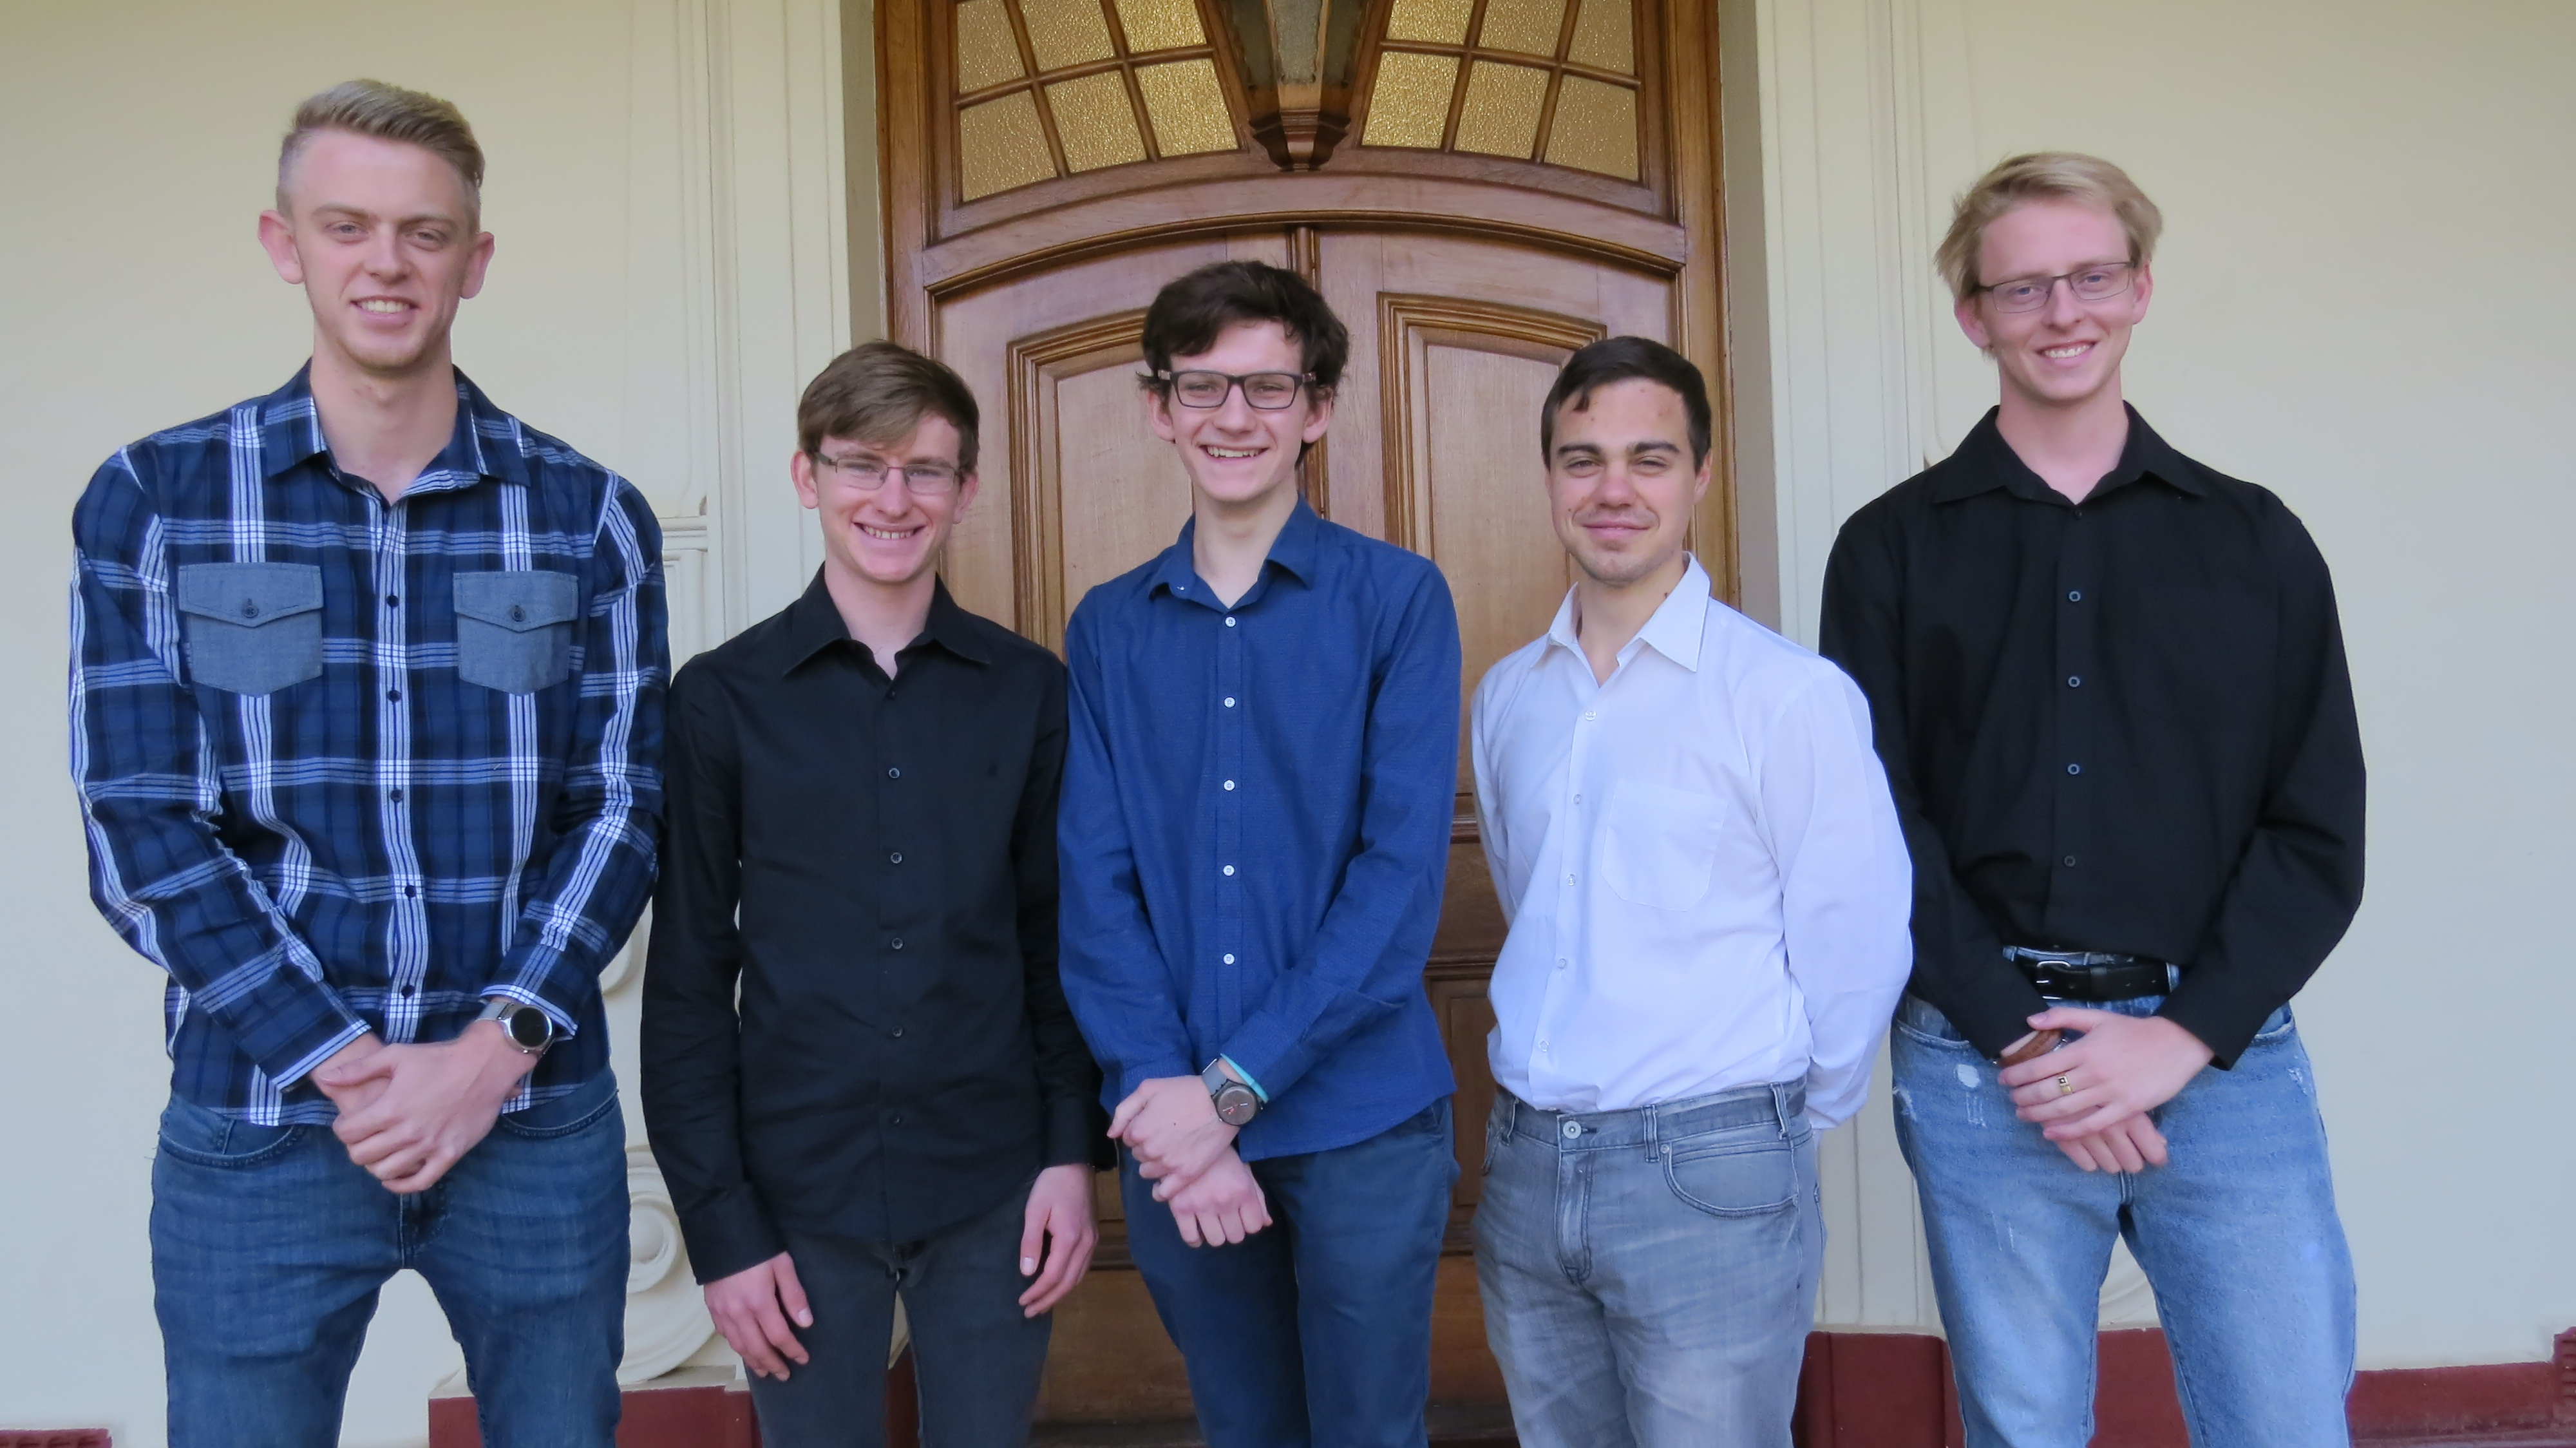
\includegraphics[width=\linewidth]{img/team_photo.jpg}}\\[2ex]
            {\large  Nicolai van Niekerk\\ \texttt{nicvaniek@gmail.com}}\\[2ex]
            {\large  Marno Hermann\\ \texttt{marno@barnton-consulting.co.za}}\\[2ex]
            {\large  Stephan Nell\\ \texttt{nellstephanj@gmail.com}}\\[2ex]
            {\large  Jan-Justin van Tonder\\ \texttt{J.vanTonder@tuks.co.za}}\\[2ex]
            {\large  Andreas Nel\\ \texttt{nel.andreas1@gmail.com}}\\[2ex]
        \end{center}
        
    \end{titlepage}
\makeatother

\cleardoublepage
\thispagestyle{empty}
\tableofcontents
\newpage

\setcounter{page}{1}

\section{Product Description}
Hutts Validation is a WebAPI that serves as an electronic ID verification system. The purpose of the system is to extract, process and validate information from a photo of an ID book, ID card or driver's license. Given a photo of the form of identification as well as given personal information, including the name, surname and a photo of the individual's face, the system will return a percentage match score for each element. This is done by validating the given information against extracted fields from the photo of the identification document. Additionally, the system can return the extracted fields given the photo of the form of identification.

\section{API Endpoints}
This section aims to give a detailed explanation of each endpoint to give the user a clear understanding of how to make a call to it, as well as what to expect from responses.
\lstset{
    string=[s]{"}{"},
    stringstyle=\color{codepurple},
    comment=[l]{:},
    commentstyle=\color{black},
}
\subsection{Extract Text}
\begin{enumerate}
	\item \textbf{Description:} Extracts textual information from the photo of the ID and returns it.
	\item \textbf{URL:} \textit{/extractText}
	\item \textbf{Method:} POST
	\item \textbf{URL Parameters:} None
	\item \textbf{Data Parameters:}

	\begin{lstlisting}
{
   "image" : [blob]
}
	\end{lstlisting}

	\textbf{Example:}

	\begin{lstlisting}
{
   "image" : idDocument.jpg
}
	\end{lstlisting}
	
	\item \textbf{Success Response:} 
		\begin{itemize}
			\item \textbf{Code:} 200
			\item \textbf{Content:}
			\begin{lstlisting}
{
   "ExtractedFields":{
   	"Surname": "Doe",
        "Names": "John Jane",
        "Sex": "M",
        "Nationality": "RSA",
        "Identity Number": "6944585228083",
        "Date of Birth": "06-05-1996",
        "Country of Birth": "RSA",
        "Status": "Citizen"
   }

}
			\end{lstlisting}
		\end{itemize}
		\item \textbf{Error Response:} TODO
		\item \textbf{Sample Call:}
		\begin{lstlisting}
$.ajax({
    type: "POST",
    url: "http://localhost:5000/extractText",
    data: {
            "image" : idDocument.jpg
          },
    success: function(data){
        console.log(data);
    }
});
		\end{lstlisting}
		\item \textbf{Notes and Comments:}
\end{enumerate}

\subsection{Extract Face}
\begin{enumerate}
	\item \textbf{Description:} Extracts the face from the photo of the ID and returns it.
	\item \textbf{URL:} \textit{/extractFace}
	\item \textbf{Method:} POST
	\item \textbf{URL Parameters:} None
	\item \textbf{Data Parameters:}

	\begin{lstlisting}
{
   "image" : [blob]
}
	\end{lstlisting}

	\textbf{Example:}

	\begin{lstlisting}
{
   "image" : idDocument.jpg
}
	\end{lstlisting}
	
	\item \textbf{Success Response:} 
		\begin{itemize}
			\item \textbf{Code:} 200
			\item \textbf{Content:}
			\begin{lstlisting}
{
   "ExtractedFace": "face.jpg"
}
			\end{lstlisting}
		\end{itemize}
		\item \textbf{Error Response:} TODO
		\item \textbf{Sample Call:}
		\begin{lstlisting}
$.ajax({
    type: "POST",
    url: "http://localhost:5000/extractFace",
    data: {
            "image" : idDocument.jpg
          },
    success: function(data){
        console.log(data);
    }
});
		\end{lstlisting}
		\item \textbf{Notes and Comments:}
\end{enumerate}

\subsection{Extract All}
\begin{enumerate}
	\item \textbf{Description:} Extracts textual information and face from the photo of the ID and returns it.
	\item \textbf{URL:} \textit{/extractAll}
	\item \textbf{Method:} POST
	\item \textbf{URL Parameters:} None
	\item \textbf{Data Parameters:}

	\begin{lstlisting}
{
   "image" : [blob]
}
	\end{lstlisting}

	\textbf{Example:}

	\begin{lstlisting}
{
   "image" : idDocument.jpg
}
	\end{lstlisting}
	
	\item \textbf{Success Response:} 
		\begin{itemize}
			\item \textbf{Code:} 200
			\item \textbf{Content:}
			\begin{lstlisting}
{
   "ExtractedData":{
   	"Surname": "Doe",
        "Names": "John Jane",
        "Sex": "M",
        "Nationality": "RSA",
        "Identity Number": "6944585228083",
        "Date of Birth": "06-05-1996",
        "Country of Birth": "RSA",
        "Status": "Citizen",
        "Face": face.jpg
   }

}
			\end{lstlisting}
		\end{itemize}
		\item \textbf{Error Response:} TODO
		\item \textbf{Sample Call:}
		\begin{lstlisting}
$.ajax({
    type: "POST",
    url: "http://localhost:5000/extractAll",
    data: {
            "image" : idDocument.jpg
          },
    success: function(data){
        console.log(data);
    }
});
		\end{lstlisting}
		\item \textbf{Notes and Comments:}
\end{enumerate}

\subsection{Verify Faces}
\begin{enumerate}
	\item \textbf{Description:} Verifies the similarity between the face on the form of identification and the photo of the individual's face.
	\item \textbf{URL:} \textit{/verifyFaces}
	\item \textbf{Method:} POST
	\item \textbf{URL Parameters:} None
	\item \textbf{Data Parameters:}

	\begin{lstlisting}
{
   "ID" : [blob],
   "face": [blob]
}
	\end{lstlisting}

	\textbf{Example:}

	\begin{lstlisting}
{
   "ID" : idDocument.jpg,
   "face": profilePic.png
}
	\end{lstlisting}
	
	\item \textbf{Success Response:} 
		\begin{itemize}
			\item \textbf{Code:} 200
			\item \textbf{Content:}
			\begin{lstlisting}
{
   "PercentageMatch": 75
}
			\end{lstlisting}
		\end{itemize}
		\item \textbf{Error Response:} TODO
		\item \textbf{Sample Call:}
		\begin{lstlisting}
$.ajax({
    type: "POST",
    url: "http://localhost:5000/verifyFaces",
    data: {
            "ID" : idDocument.jpg,
            "face": profilePic.png
          },
    success: function(data){
        console.log(data);
    }
});
		\end{lstlisting}
		\item \textbf{Notes and Comments:}
\end{enumerate}

\subsection{Verify Info}
\begin{enumerate}
	\item \textbf{Description:} Verifies the similarity between the text on the form of identification and the provided personal information.
	\item \textbf{URL:} \textit{/verifyInfo}
	\item \textbf{Method:} POST
	\item \textbf{URL Parameters:} None
	\item \textbf{Data Parameters:}

	\begin{lstlisting}
{
    "surname": [string],
    "names": [string],
    "gender": [string],
    "nationality": [string],
    "idNumber": [string],
    "dob": [date],
    "cob": [string],
    "satus": [string],
    "idPhoto": [blob]
}
	\end{lstlisting}

	\textbf{Example:}

	\begin{lstlisting}
{   
    "surname": "Doe",
    "names": "John Joe",
    "gender": "M",
    "nationality": "South African",
    "idNumber": "9877452008082",
    "dob": "1998-07-06",
    "cob": "RSA",
    "satus": "Citizen",
    "idPhoto": myId.jpg
}
	\end{lstlisting}
	
	\item \textbf{Success Response:} 
		\begin{itemize}
			\item \textbf{Code:} 200
			\item \textbf{Content:}
			\begin{lstlisting}
{
   "PercentageMatch": 96
}
			\end{lstlisting}
		\end{itemize}
		\item \textbf{Error Response:} TODO
		\item \textbf{Sample Call:}
		\begin{lstlisting}
$.ajax({
    type: "POST",
    url: "http://localhost:5000/verifyInfo",
    data: {
            "surname": "Doe",
            "names": "John Joe",
            "gender": "M",
            "nationality": "South African",
            "idNumber": "9877452008082",
            "dob": "1998-07-06",
            "cob": "RSA",
            "satus": "Citizen",
            "idPhoto": myId.jpg
          },
    success: function(data){
        console.log(data);
    }
});
		\end{lstlisting}
		\item \textbf{Notes and Comments:}
\end{enumerate}

\subsection{Verify ID}
\begin{enumerate}
	\item \textbf{Description:} Verifies the similarity between the text and image on the form of identification and the provided personal information with a photo of the individual's face.
	\item \textbf{URL:} \textit{/verifyID}
	\item \textbf{Method:} POST
	\item \textbf{URL Parameters:} None
	\item \textbf{Data Parameters:}

	\begin{lstlisting}
{
    "userImage": [blob],
    "surname": [string],
    "names": [string],
    "gender": [string],
    "nationality": [string],
    "idNumber": [string],
    "dob": [date],
    "cob": [string],
    "satus": [string],
    "idPhoto": [blob]
}
	\end{lstlisting}

	\textbf{Example:}

	\begin{lstlisting}
{   
    "userImage": profilePic.png,
    "surname": "Doe",
    "names": "John Joe",
    "gender": "M",
    "nationality": "South African",
    "idNumber": "9877452008082",
    "dob": "1998-07-06",
    "cob": "RSA",
    "satus": "Citizen",
    "idPhoto": myId.jpg
}
	\end{lstlisting}
	
	\item \textbf{Success Response:} 
		\begin{itemize}
			\item \textbf{Code:} 200
			\item \textbf{Content:}
			\begin{lstlisting}
{
   "PercentageMatch": 61
}
			\end{lstlisting}
		\end{itemize}
		\item \textbf{Error Response:} TODO
		\item \textbf{Sample Call:}
		\begin{lstlisting}
$.ajax({
    type: "POST",
    url: "http://localhost:5000/verifyInfo",
    data: {
            "userImage": profilePic.png,
            "surname": "Doe",
            "names": "John Joe",
            "gender": "M",
            "nationality": "South African",
            "idNumber": "9877452008082",
            "dob": "1998-07-06",
            "cob": "RSA",
            "satus": "Citizen",
            "idPhoto": myId.jpg
          },
    success: function(data){
        console.log(data);
    }
});
		\end{lstlisting}
		\item \textbf{Notes and Comments:}
\end{enumerate}

\end{document}